%!TEX root = Report.tex

\subsection{Experimentation with ants}
\label{ants}

During this project we had to decide whether to paint the ants or not, and if so what color. Figure \ref{fig:antcoloring} shows four examples of ants, with both their natural color, shown in image \emph{a}, and painted versions shown in image \emph{b}(red), \emph{c}(green) and \emph{d}(white). The images are recorded using the webcam from the plotter. We can see from these image that coloring an ant is preferred. Painting it white gives the best contrast compared to the background. Furthermore we suggest putting the ant to be painted in a freezer for 2-4 minutes as this will put it in a sedated state, making it much easier to paint. After a couple of minutes it will act normal again.\\

\begin{figure}
        \centering
        \begin{subfigure}[b]{0.35\textwidth}
                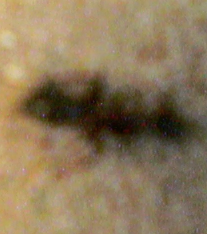
\includegraphics[scale = 0.5]{img/natural_ant}
                \caption{}
        \end{subfigure}
		\quad
        \begin{subfigure}[b]{0.35\textwidth}
                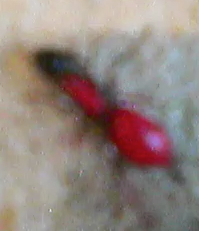
\includegraphics[scale = 0.5]{img/red_ant}
                \caption{}
        \end{subfigure} \hfill \\ \mbox{}\\
        \begin{subfigure}[b]{0.35\textwidth}
                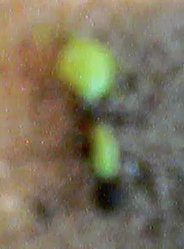
\includegraphics[scale = 0.5]{img/green_ant}
                \caption{}
        \end{subfigure}
		\quad
        \begin{subfigure}[b]{0.35\textwidth}
                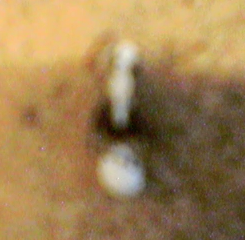
\includegraphics[scale = 0.5]{img/white_ant}
                \caption{}
        \end{subfigure}
        \caption{Coloring ants in different colors}
		\label{fig:antcoloring}
\end{figure}

A second problem were to keep the ant within the petri dish. The ant had no problem climbing the sides of the petri dish and escape. We therefore tried several different solutions to keep them. We were adviced to try teflon tape on the sides of the petri dish, as they should not be able to climb the slippery surface of that tape. This did not prove successful so we tried other types of slippery tape versions like silicone and wax tapes. See the different types of tape in Figure \ref{fig:tape}. Unfortunately none of them were able to solve our problem. We were also adviced to use mineral oil, however we were unable to get a hold of any such oil. We tried with cooking oil instead such as sunflower oil and olive oil, however they did not have the desired effect.\\

\begin{figure}[ht!]
  \centering
    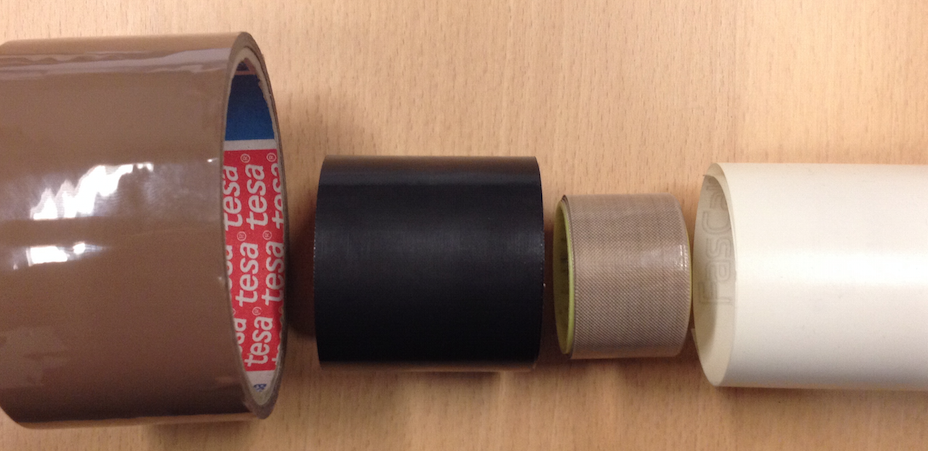
\includegraphics[scale=0.25]{img/tape}
  \caption{Different types of slippery tape used}
  \label{fig:tape}
\end{figure}

We followed up by trying to use natural ant repellents such as kitchen salt, however our tests did not prove fruitful as it did not have any effect.\\

Our solution was to eleminate all sides completely and create an "island" instead. We filled the petri dish with dirt until it was completely full, and placed it within a much larger petri dish full of water. We hoped that the ant would not cross the water, and thereby stay in the inner petri dish during our tests. The setup can be seen in Figure \ref{fig:petridish}. This solution proved much more successful, as the ant did not move into the water immedietly. However after some time it realized that it was completely surrounded by water, and try to swim away. It would take a long time for the ant to try this, giving us enough time to test our software.\\

\begin{figure}[ht!]
  \centering
    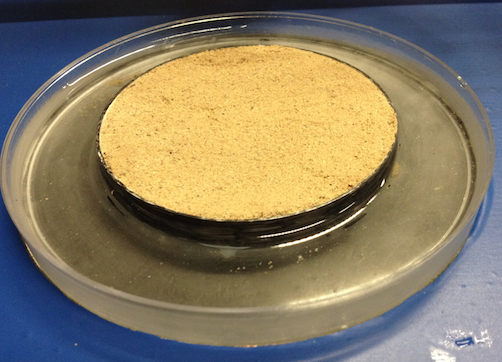
\includegraphics[scale=0.25]{img/petridish}
  \caption{}
  \label{fig:petridish}
\end{figure}